\label{sub:gtx_state_of_the_art}
Looking for a subgraph $H$ of $G$ that best preserve the distance in $G$ while being sparse is an old
problem, especially driven by network design in fields such as transportation~\autocite{RoadNetworks60}
and electrical circuits~\autocite{electricalNetworks60}. For instance, \textcite{Johnson1978} define
the following problem\footnote{We adapt their notations to match ours}:  
\begin{problem}[Network Design Problem]
  \label{prob:gtx_ndp}
  Given an undirected integer-weighted graph $G=(V, E, w)$, a budget $B\in\Nbb$ and a criterion
  threshold $C\in \Nbb$, does there exist a spanning subgraph $G'=(V, E')$ of $G$ with weight
  $w(E') \leq B$ and criterion value $F(G') \leq C$, where the criterion function $F(G')$ denotes
  the sum of the weights of the shortest paths in $G'$ between all vertex pairs?
\end{problem}
Note that their definition of stretch includes all possible edges in $G$ and not only those in $E$.
They prove that this problem is \NPc{} by exhibiting a reduction from the \textsc{Knapsack}
problem. Finally they prove that the simpler problem of finding a spanning tree on an unweighted
graph, that is
\vspace{-.5\baselineskip}
\begin{problem}[Simple Network Design Problem]
  \autoref{prob:gtx_ndp} with $w$ being the equal to $1$ for all edges in $E$ and $B=|V|-1$.
\end{problem}%
\vspace{-.5\baselineskip}
\noindent is also \NPc{} by reduction from \textsc{Exact 3-Cover}.
In this setting of a spanning tree minimizing the stretch over all pairs of nodes, \enquote{
\textcite{AllPairStrech08} obtained a $(c log n)^{O(\log \Delta)}$ factor, where $c$ is the optimal
maximum stretch and $\Delta$ is the diameter.  They also showed $O(1)$ approximation for the case
where the graph is unweighted. The constant was later reduced to $6$ by \textcite{AllPairStrech10}}

\begin{problem}[Optimal Communication Spanning Tree~\autocite{Requirements74}]
Given a set of nodes $V=\{v_1, \ldots, v_n\}$, a set of distances $d_{ij}$ and a set of requirements
$r_{ij}$ between $v_i$ and $v_j$, find a spanning tree connecting these $n$ nodes such that the
total cost of communication of the spanning tree is a minimum among all spanning trees. The cost of
communication for a pair of nodes is $r_{i,j}$ multiplied by the sum of the distances of arcs which
form the unique path connecting $v_i$ and $v_j$ in the spanning tree. The cost of a spanning tree is
the sum of costs over all pairs of nodes.
\end{problem}

Given a weighted graph $G=(V,E,w)$, if we let $d_{ij}$ be $w((i,j))$ and $r_{ij}$ be $1$ if
$(i,j)\in E$ and $0$ otherwise, it seems to me this correspond to the weighted low stretch problem.
% However, \textcite[Section 3, page 453]{lognMetricBoundConf03} claim a $O(\log n)$ approximation so maybe I'm
% wrong. Turns out, they refer to a distribution over trees and this $O(\log n)$ is the expected
% stretch of a tree sampled from this distribution

This defines two kind of structures, spanning trees and spanners (which are still sparse subgraphs
yet containing more than $|V|-1$ edges).

\paragraph{Trees}
\label{par:trees}

Earlier but slightly less related, \textcite{OptimalNetwork69} studies the following problem:
\begin{problem}[Optimal Network Problem]
  \label{prob:gtx_scott}
  Given a set $V$ of $n$ vertices, find a set of spanning edges $E\subset V^2$ that minimizes
  the sum of the length of the shortest paths  between all vertex pairs while the
  total length of the resulting network does not exceed some upper bound $B\in\Nbb$.
\end{problem}
This can be seen as a special case of \autoref{prob:gtx_ndp} with $G$ being the unweighted
\marginpars{according to the experiments, it's not clear whether there are weights or
not…} $n$-complete graph. He proposes a backtracking solution and two local search approximate
algorithms. Some early branch and bound heuristic solutions to \autoref{prob:gtx_scott} are surveyed
in~\autocite[Section 2.3.2]{networkDesignSurvey89} although they do not come with asymptotic
guarantee on the stretch. Furthermore, \textcite{optimApproxNP80} proves that for any $\epsilon \in
(0,1)$, finding a $|V|^{1-\epsilon}$ approximation is \NPc{}.

Next is the seminal paper of \textcite{LowerBound95}. It touches on many topics, and frame the
problem in a game theoretic way but here we only focus on two of their results: a lower bound of
$\Omega(\log n)$ for the average stretch of any tree and their construction of a tree with $\exp
O(\sqrt{\log n\log\log n})$ average stretch in time $O(m^2)$. The lower bound follows from an
existing result in extremal graph theory~\autocite[pages 107--109]{ExtremalGraph04}: there is a
positive constant $a$ such that for all $n\in \Nbb$, one can construct a graph $G$ with $n$ vertices
and $2n$ edges such that every cycle $G$ has a length of at least $a\log n$. Now consider any
spanning tree $T$ of $G$.  While all the $n-1$ edges of $T$ have a stretch of $1$, the $n+1$
remaining ones form a cycle in $T$ hence in $G$ as well and thus incur a stretch of at least $a\log
n$. This shows that the average stretch is at least $\frac{1}{2}a\log n$.

They construct a low stretch spanning tree in a bottom up manner like the \gtx{} algorithm. First,
they extend the definition of stretch to multigraph~\autocite[Section 4]{LowerBound95} and then
describe a procedure to transform in linear time any multigraph $G$ with $n$ nodes to a multigraph
$G'$ on the same nodeset with at most $n(n+1)$ edges such the average stretch of $G'$ is at most
twice that of $G$~\autocite[Lemma 5.2]{LowerBound95}. The next ingredient is an algorithm to build a
low diameter decomposition of a multigraph $G$, parametrized by a number $x(n)$ depending of $n$. It
works by repeatedly selecting an arbitrary node and growing a ball around it until the number of
edges leaving the ball is at most a fraction $\nicefrac{1}{x(n)}$ of the number of edges with both
endpoints in the ball. The key property of this decomposition is that it yields a partition of $G$
in clusters such that the radius of each cluster is small (namely at most $O(x(n)\log n)$) and there
is most a fraction $\nicefrac{1}{x(n)}$ of edges between clusters. Finally, the iterative procedure
is a follows: once a partition has been built, we compute a shortest path spanning tree in each
cluster that are then collapsed into super nodes to form the next graph $G'$ and the process repeats.
Another difference from \gtx{}, besides the partition procedure, is that $G'$ is a multigraph,
taking into account the number of edges joining cluster, while \collapseStar{} picks only the most
direct one.

Another interesting idea from this paper is to consider a distribution over trees instead of a
single instance, especially when one is concern about the maximum stretch instead of the average
one. For instance, on a cycle with $n$ nodes, a tree is obtained by removing one edge, and that edge
incurs a stretch of $n-1$. The uniform distribution over such trees has a maximum stretch of
$2\left(1 - \frac{1}{n}\right)$~\autocite{circle2k89}.

\begin{table}[htbp]
  \centering
  \caption{Reproduction of Table 1 from~\autocite{Abraham2012} showing the evolution of the best
  asymptotic average stretch over time.}\label{tab:gtx_related}
  \begin{tabular}{lll}
    \toprule
    work                      & average stretch                          & time                    \\
    \midrule
    \autocite{LowerBound95}   & $\exp(O(\sqrt{\log n\log\log n}))$       & $O(m^2)$                \\
    \autocite{LowerStretch05} & $O((\log n)^2 \log \log n)$              & $O(m \log^2 n)$         \\
    \autocite{nearlyTight08}  & $O(\log n(\log \log n)^3)$              & $O(m \log^2 n)$         \\
    % \autocite{nearlyTight08}  & $O(\log n \log\log n(\log\log\log n)^3)$ & $O(m^2)$                \\
    \autocite{TighterSDD11}   & $O(\log n(\log \log n)^3 )$              & $O(m \log n\log\log n)$ \\
    \autocite{Abraham2012}    & $O(\log n \log \log n)$                  & $O(m \log n\log\log n)$ \\
    \bottomrule
  \end{tabular}
\end{table}

\autocite{LowerStretch05} is the star decomposition described in section 3 of \autocite{papplow},
which was modified by \autocite{nearlyTight08} to improve the stretch. Then \textcite{TighterSDD11}
improved the runtime by rounding the edge weights to the closest power of $2$ and using a modified
implementation of the Dijkstra's algorithm in the case of at most $k$ distinct edge
weights~\autocite{FastPathFewWeights10}. Finally, \textcite{Abraham2012} describe an even more
complex but tighter petal decomposition.
\begin{marginfigure}
  \centering
  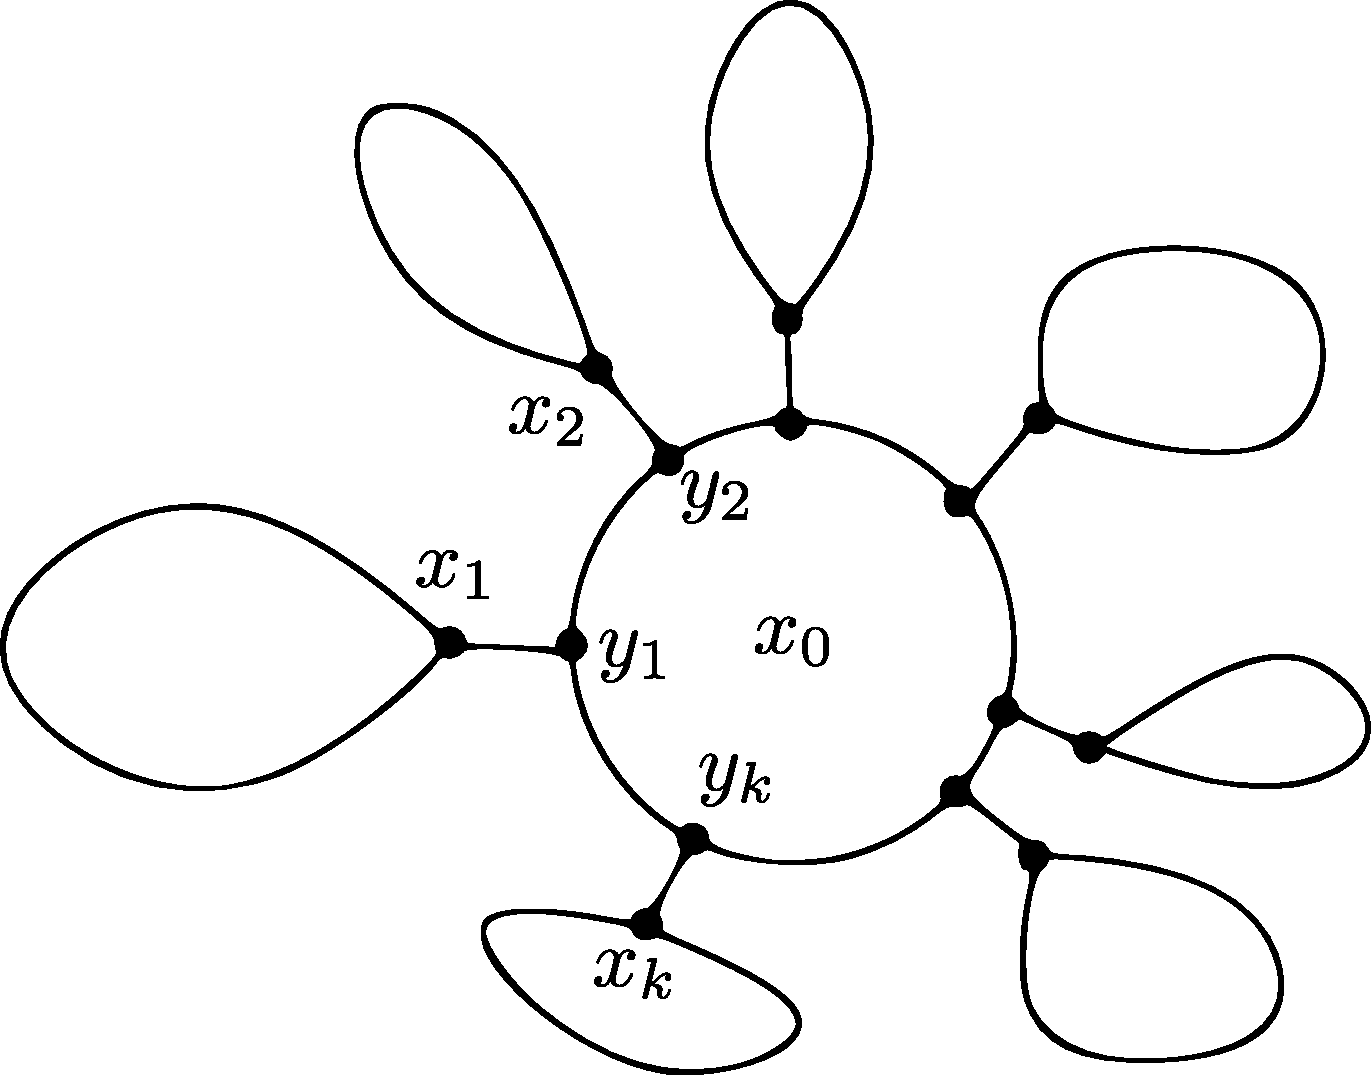
\includegraphics[width=.95\textwidth]{assets/raw/star_decomp.pdf}
  \caption{Star decomposition (reproduced from Figure 1 of~\autocite{LowerStretch05})}
  \label{fig:gtx_star_decomp}
\end{marginfigure}


If the tree is non spanning (\ie{} it can include edges not from the original graph as long as the
distances in tree remain larger the distances in the graph), the average stretch can be reduced to
$\Theta(\log n)$~\autocite{lognMetricBoundConf03}. Furthermore, when the objective if to minimize
the average stretch over all possible pairs of node, then \textcite{constantDistortion07} achieve a
universal constant bound.

Special case of graph
series parallel
\enquote{In a subsequent paper, \textcite{seriesParallel06} proved that every series-parallel
unweighted graph admits a spanning tree of average stretch $O(log n)$. This bound is tight as it
matches the lower bound established in~\autocite{cutsTrees99}.}

more special cases are in~\autocite{specialCase14}, although it's for the minimum max stretch
$t^\star$.
\enquote{Note also that a number of particular graph classes (like interval
graphs, permutation graphs, asteroidal-triple–free graphs, strongly chordal graphs,
dually chordal graphs, and others) admit tree $t$-spanners for small values of $t$}

A tangential problem is \enquote{Light Approximate Shortest-path Trees (LASTs).  Given a set of
“sources” and a sink, a LAST is a tree of weight close to the minimum spanning tree (MST) on the
sources and the sink, such that the tree distance from any source to the sink is close to the
shortest-path distance. Khuller, Raghavachari, and Young (KRY95) defined and studied LASTs in the
offline setting and showed that one can get constant stretch with cost constant times the
MST.}\footnote{FOCS'17 \href{https://arxiv.org/abs/1611.00052}{arxiv.org/abs/1611.00052}}

\paragraph{Spanners}
\label{par:spanners}

\url{http://www.siam.org/meetings/da17/schedule.html} SODA 13B \url{http://dl.acm.org/citation.cfm?id=3039686}
for instance the Elkin paper~\autocite{Spanner17} \enquote{Our centralized randomized algorithm computes (with
probability close to 1), a $(2k - 1)$-spanner with $n \cdot (1 + O(\frac{\log k}{n}))$ edges in
$O(|E|)$ time, whenever $k = \Omega(\log n)$. Note that when $k = \omega(\log n)$, the number of
edges is $n(1+o(1))$, i.e., in this range the algorithm computes an ultra-sparse spanner in $O(|E|)$
time.} For instance, if $k=5\log n$, we get a $10\log n$-spanner with $n\left(1+O\left(\frac{\log\log
n}{n}\right)\right)$ edges in $O(|E|)$ time.

the subgraph $H$ is said to be an $(\alpha, \beta)$-spanner of $G$ if, for a pair of parameters
$\alpha \geq 1$, $\beta \geq 0$, and for every pair $u, v \in V$ of vertices, it holds that $d_H(u,
v) \leq \alpha\cdot d_G(u, v)+\beta$.

They have applications in computing approximately shortest
paths [9, 22, 28, 37], routing [48], distance oracles and
labeling schemes [49, 56, 36] and synchronization [7].

From 6:They also appear in biology in the process of reconstructing phylogenetic trees from
matrices, whose entries represent genetic distances among contemporary living species (H. J.
Bandelt, A. W. M. Dress, Reconstructing the Shape of a Tree from Observed Dissimilarity Data, Adv.
in Appl. Math. 7 (1986)). Robotics researchers have studied spanners under the constraints of
Euclidean geometry, where vertices of the graph are points in space, and edges are line segments
joining pairs of points (Chew), (Dobkin), $[DJ], [K], [KG], [LL]$. 

studied in 1; 4; 6; 9; 15; 19; 22; 24; 26; 28; 30; 31; 37; 43; 51; 52; 57; 58



\begin{tabulary}{\textwidth}{LLLLL}
  \toprule
  work  & average stretch & edge size                              & weighted & time                                             \\
  \midrule
  46    & $4k + 1$        & $O(n^{1+\nicefrac{1}{k}})$             & no       & polynomial                                       \\
  6     & $2k +1$         & $O(n\cdot \ceil{n^{\nicefrac{1}{k}}})$ & yes      & $O\left(m(n^{1+\nicefrac{1}{k}}+n\log n)\right)$ \\
  40    & $2k-1$          & $O(n^{1+\nicefrac{1}{k}}+n)$           & no       & $O(m)$                                           \\
  Elkin & $2k-1$          & $n \cdot (1 + O(\frac{\log k}{n}))$    & no       & $O(m)$                                           \\
  \bottomrule
\end{tabulary}

% 22: E. Cohen, "Fast algorithms for constructing t-spanners and paths with stretch t," Proceedings
% of 1993 IEEE 34th Annual Foundations of Computer Science, Palo Alto, CA, 1993, pp. 648-658.  doi:
% 10.1109/SFCS.1993.366822
% We construct t-spanners of size (number of edges) Õ(n 1+(2+\epsilon)/t )
% (for any \epsilon > 0 and t such that t/(2+\epsilon) is integral). These spanners can be constructed
% by a randomized algorithm that runs in Õ(mn (2+\epsilon)/t ) time.


% Halperin and Zwick [40].  Their deterministic algorithm, for an integer parame- ter k ≥ 1,
% computes a (2k − 1)-spanner with n 1+1/k + n edges in O(|E|) time. (Their result improved previous
% pioneering work by [46, 22].)

Describe the greedy algorithm of 6. Using (55 On Dynamic Shortest Paths Problems Liam Roditty, Uri
Zwick, 2004), it runs in $O(\alpha n^{2+\nicefrac{1}{\alpha}})$

peleg 2007 hardness results

46: Peleg, D. and Schäffer, A. A. (1989), Graph spanners. J. Graph Theory, 13: 99–116.
doi:10.1002/jgt.3190130114

study the problem on unweighted graph. Application to routing scheme (48: D. Peleg and E. Upfal, A
tradeoff between space and efficiency for routing tables. 20th ACM Symposium on the Theory of
Computing, Chicago (1988))
Special case for the complete graph weighted by the distance in a 2D plan. Existing $\sqrt{10}$
spanner for the $\ell_1$ metric (L. P. Chew, There is a planar graph almost as good as the complete
graph.  Proceedings of the 2nd ACM Symposium on Computational Geometry, (1986)) (improved to
$\sqrt{4+2\sqrt{2}}$ by N. Bonichon, C. Gavoille, N. Hanusse, L. Perkovic The stretch factor of
$\ell_1$ and $\ell_{\infty}$ Delaunay triangulations European Symposium on Algorithms (ESA) (2012))
and $\phi \pi$ for $\ell_2$ (D. P. Dobkin, S. J. Friedman, and K. J. Supowit, Delaunay graphs are
almost as good as complete graphs. 28th IEEE Symposium on the Foundations of Computer Science,
(1987)) (improved to $1.998$ by Ge Xia. 2011. Improved upper bound on the stretch factor of delaunay
triangulations. In Proceedings of the twenty-seventh annual symposium on Computational geometry
(SoCG '11)). See (Prosenjit Bose, Michiel Smid, On plane geometric spanners: A survey and open
problems, Computational Geometry, Volume 46, Issue 7, 2013) for more on the 2D case.
In undirected graph, finding a spanner with less than $k$ edges is \NPc{} (theorem 2.2)
For $k<n$, one can construct in polynomial time a $(4\log_k n +1)$ spanner with less than $kn$ edges
(theorem 2.4) giving for instance ($k=2$) $O(\log n)$ spanner with $O(n)$ edges and
($k=n^{\nicefrac{1}{r}}$, $r\geq 1$) a $(4r+1)$ spanner with $O(n^{1+\nicefrac{1}{r}})$ edges
(matching lower bound within constant factor). For every $d \geq 0$, the $d$-dimensional cube has a
$3$-spanner with fewer than $7\time 2^d$ edges (Lemma 2.10 from 47: D. Peleg and J. D. Ullman. An
optimal synchronizer for the hypercube. SIAM J. on Comput., 18:740–747, 1989)
For chordal graphs: for every $n$-vertex chordal graph there exists a $2$-spanner with
$O(n\sqrt{n})$ edges (matching lower bound), a $3$-spanner with $O(n \log n)$ edges and a $5$-spanner
with $O(n)$ edges.
Much more difficult for directed graph, according to Theorem 4.2: For every $t \geq 1$ there are
infinitely many $n$-vertex directed graphs for which every $t$-spanner requires
$\Omega(\nicefrac{n^2}{t^2})$ edges.

% check some surveys of the 80's
% http://pubsonline.informs.org/doi/abs/10.1287/trsc.18.1.1
% http://onlinelibrary.wiley.com/doi/10.1002/net.3230190305/full
% early solutions
% http://onlinelibrary.wiley.com/doi/10.1002/net.3230090104/full
% http://onlinelibrary.wiley.com/doi/10.1002/net.3230130309/full
% later solution?
% http://ieeexplore.ieee.org/document/81738


While they have many applications [see first paragraph of \url{https://arxiv.org/pdf/1401.2454.pdf},
which was later merged in a STOC'14 paper] (a major one being solving linear systems), in some
practical situations their advantages are less clear [from
\url{https://link.springer.com/chapter/10.1007/978-3-319-20086-6_16}\enquote{for reasonable inputs
the constant factors make the solver much slower than methods with higher asymptotic complexity.
One other aspect predicted by theory is confirmed by our findings: Spanning trees with lower
stretch indeed reduce the solver's running time. Yet, simple spanning tree algorithms perform
better in practice than those with a guaranteed low stretch.} this is improved by
\url{https://link.springer.com/chapter/10.1007%2F978-3-319-20086-6_17} although they seem to work
	mostly with the Laplacian of the tree ]
